\documentclass[11pt]{article}

\usepackage[a4paper,margin=3cm]{geometry} % For page dimensions
\usepackage{fontspec} % For font selection
\usepackage{unicode-math} % For mathematical fonts
\usepackage{polyglossia} % For language selection
\usepackage{graphicx} % For images
\usepackage[colorlinks=true, linkcolor=black, urlcolor=blue, citecolor=green]{hyperref} % For hyperlinks
\usepackage{xcolor} % Colors for code highlighting
\usepackage{fancyhdr} % For headers and footers
\usepackage{bookmark}
% \usepackage{draftwatermark} % For watermarks

\usepackage{amsmath} % For mathematical equations
\usepackage{listings} % For code formattings
\usepackage{tikz} % For diagrams

\graphicspath{ {images} }

% Set fonts
% \setmainfont{Noto Serif}
\setromanfont{Noto Serif}
\setsansfont{Noto Sans}
\setmonofont{Noto Sans Mono}

% Set languages
\setmainlanguage{greek}
\setotherlanguages{english}

% Watermark
% \SetWatermarkScale{1}
% \SetWatermarkColor{gray}
% \SetWatermarkLightness{0.5}

% Header and footer settings
\pagestyle{fancy}
\setlength{\headheight}{14pt}
\fancyhf{}
\fancyhead[L]{ParkOut}
\fancyhead[R]{\leftmark} % section name
\fancyfoot[C]{\thepage}

\newcommand{\email}[1]{\href{mailto://#1}{\texttt{#1}}} % Email formatting

\begin{document}
\begin{titlepage}
    \centering
    \Huge
    ParkOut \\
    \normalsize
    \vspace{1cm}
    % TODO project logo
    % \includegraphics[width=0.5\textwidth]{upatras-logo.jpg}
    % \vspace{1cm}
    \begin{tabular}{cc}
        Γιάννης Ραβασόπουλος            & Κώστας Λουκανάρης               \\
        1100696                         & 1100610                         \\
        \email{up1100696@ac.upatras.gr} & \email{up1100610@ac.upatras.gr} \\
        \\
        Χρήστος Μάριος Νικολόπουλος     & Άγγελος Αβεντισιάν              \\
        1100644                         & 1100491                         \\
        \email{up1100644@ac.upatras.gr} & \email{up1100491@ac.upatras.gr} \\
        \\
    \end{tabular} \\
    Βασίλης Μυλωνάς \\
    1100643 \\
    \email{up1100643@ac.upatras.gr} \\
    \vspace{1.5cm}
    \Large
    \today \\
    \vspace{0.5cm}
    Τεχνολογία Λογισμικού \\
    \vspace{0.5cm}
    Τμήμα Μηχανικών Η/Υ και Πληροφορικής, \\
    Πανεπιστήμιο Πατρών \\
    \normalsize
\end{titlepage}

\newpage

\begin{abstract}
    Ανάπτυξη συστήματος και συνοδεύουσας εφαρμογής για την εύρεση/ενοικίαση
    θέσεων στάθμευσης και την διευκόλυνση συνεπιβίβασης σε κοινές διαδρομές.
    Η εφαρμογή εγκαθισταται σε κινητές συσκευές και παρέχει ζωντανή πληροφόρηση
    αντλώντας πληροφορίες από τους χρήστες, στατιστικά μοντέλα και από δίκτυα
    αισθητήρων\footnote{Μελλοντική λειτουργία} όπου αυτό είναι δυνατό. Η
    εφαρμογή απευθύνεται αμφότερα σε οδηγούς αυτοκινήτων αλλά και σε πεζούς.
    Στόχος είναι η καλύτερη αξιοποίηση του οδικού δικτύου και η μείωση της
    κυκλοφοριακής συμφόρησης σε αστικές περιοχές.
\end{abstract}

\newpage

\tableofcontents

\newpage

\section{Σύσταση Ομάδας}

Η ομάδα αποτελείται από 5 μέλη:

\begin{itemize}
    \item Βασίλης Μυλωνάς (Επικεφαλής Έργου/Project Manager)
    \item Άγγελος Αβεντισιάν (Υπεύθυνος Ποιότητας/QA Manager)
    \item Γιάννης Ραβασόπουλος
    \item Κώστας Λουκανάρης
    \item Χρήστος Μάριος Νικολόπουλος
\end{itemize}

\newpage

\section{Domain Model}

\begin{description}
    \item[User]
        Οποιοσδήποτε χρήστης της εφαρμογής. Με αυτόν τον όρο περιγράφουμε
        οποιοδήποτε άτομο, επιχείρηση ή άλλη οντότητα που αξιοποιεί τις
        υπηρεσίες της εφαρμογής.
    \item[Driver]
        Ένας χρήστης της εφαρμογής ο οποίος οδηγεί κάποιο όχημα.
    \item[Vehicle]
        Ένα όχημα που χρησιμοποιείται για μετακίνηση από κάποιον οδηγό της
        εφαρμογής.
    \item[ParkingSpace]
        Ένας γενικευμένος χώρος στάθμευσης. Μπορεί να είναι δημόσιος ή ιδιωτικός
        π.χ. ένα τμήμα δρόμου, ένα γκαράζ που νοικιάζει κάποιος ή ένας υπόγειος
        χώρος.
    \item[ParkingSpot]
        Μια συγκεκριμένη θέση στάθμευσης. Μπορεί να είναι διαθέσιμη,
        κατειλημμένη ή σε άγνωστη κατάσταση. Μια θέση στάθμευσης είναι πάντα
        μέρος ενός χώρου στάθμευσης.
    \item[ParkingReservation]
        Μια κράτηση μιας θέσης στάθμευσης. Αφορά κυρίως ιδιωτικούς χώρους
        στάθμευσης. Eίναι έναντι πληρωμής και μπορεί να είναι
        προγραμματισμένη ή άμεση.
    \item[ParkingSpaceOwner]
        Ένας χρήστης της εφαρμογής ο οποίος είναι ιδιοκτήτης ενός χώρου
        στάθμευσης και το έχει δηλώσει μέσω της εφαρμογής. Μπορεί να
        είναι ιδιώτης ή κάποια επιχείρηση π.χ. ένας
        ιδιοκτήτης πολυκατοικίας ο οποίος ενοικιάζει τον υπόγειο χώρο στάθμευσης
        σε τρίτους μέσω της εφαρμογής ή μια εταιρεία που διαχειρίζεται ένα
        πολυόροφο χώρο στάθμευσης.
    \item[Payment]
        Μια πληρωμή που πραγματοποιείται μέσω της εφαρμογής. Ενδεικτικά μπορεί
        να αφορά την ενοικίαση μιας θέσης στάθμευσης ή την αγορά ενός
        εισιτηρίου για παρκόμετρο.
    \item[Rating]
        Η βαθμολογία που δίνει ένας χρήστης σε έναν άλλο χρήστη. Μπορεί να
        αφορά την συμπεριφορά του χρήστη ή την κατάσταση ενός χώρου
        στάθμευσης. Μπορεί να περιλαμβάνει σχόλια και εικόνες.
    \item[Report]
        Μια αναφορά που κάνει ένας χρήστης σε έναν άλλο χρήστη για να
        καταγγείλει παράνομη η ανεπιθύμητη δραστηριότητα. Περιλαμβάνει
        κείμενο και έναν λόγο αναφοράς.
    \item[Location]
        Μια γεωγραφική τοποθεσία, περιλαμβάνει διεύθυνση ή συντεταγμένες.
    \item[Route]
        Μια διαδρομή από ένα σημείο Α σε ένα σημείο Β. Μπορεί να περιλαμβάνει
        σημεία στάσης.
    \item[Ride]
        Αντιπροσωπεύει μια συνεπιβίβαση. Ένας οδηγός εκτελώντας μια διαδρομή
        μπορεί να μεταφέρει περισσότερους από έναν επιβάτες οι οποίοι έχουν
        κοινό προορισμό.
    \item[Pickup]
        Αντιπροσωπεύει την παραλαβή ενός επιβάτη από τον οδηγό. Περιλαμβάνει
        σημείο συνάντησης και ώρα.
    \item[Carpooler]
        Ένας χρήστης της εφαρμογής ο οποίος δεν οδηγεί κάποιο όχημα αλλά
        χρησιμοποιεί τις υπηρεσίες της εφαρμογής για να βρει οδηγούς που πάνε
        στο ίδιο μέρος με αυτόν.
    \item[Area]
        TODO
    \item[Reward]
        Μια επιβράβευση η οποία δίνεται σε έναν χρήστη με βάση την χρήση της
        εφαρμογής. Για παράδειγμα ένας οδηγός που μεταφέρει πολλούς επιβάτες
        μπορεί να λάβει ένα κουπόνι έκπτωσης 15\% σε κάποιον φούρνο.
\end{description}

\begin{figure}
    \centering
    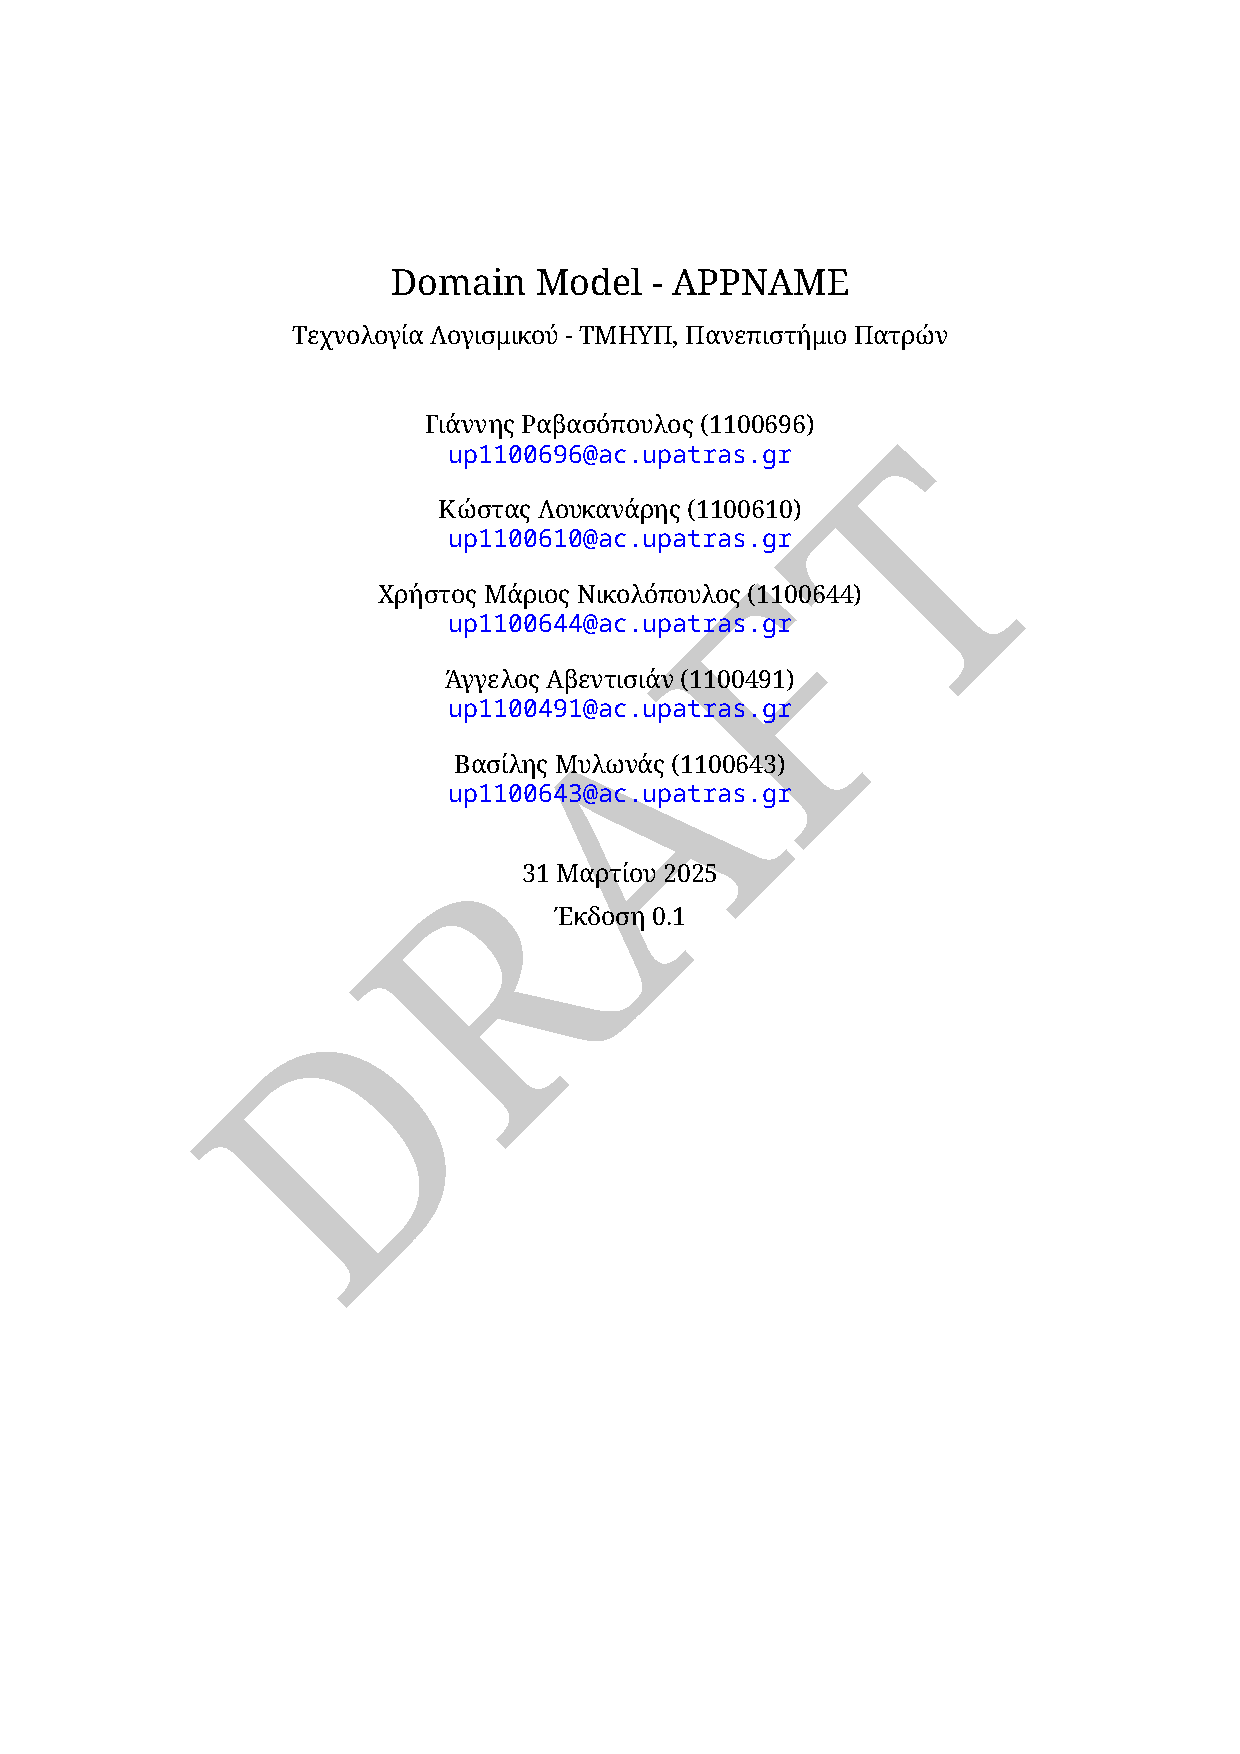
\includegraphics[width=\textwidth]{domain-model}
    \caption{Domain Model}
\end{figure}

\newpage

\section{Use Cases}

\subsection{Redeem Reward}

Ο χρήστης επιθυμεί να λάβει μια ανταμοιβή που έχει κερδίσει μέσω
της εφαρμογής.

\subsubsection{Βασική Ροή}

\begin{enumerate}
    \item Ο χρήστης επιλέγει "Redeem Reward"
    \item Η εφαρμογή υπολογίζει τους πόντους του χρήστη.
    \item Η εφαρμογή εμφανίζει τις διαθέσιμες ανταμοιβές και τους πόντους.
    \item Ο χρήστης επιλέγει την ανταμοιβή που επιθυμεί.
    \item Η εφαρμογή ενημερώνει τους πόντους του χρήστη και αφαιρεί την ανταμοιβή
          από τη λίστα των διαθέσιμων ανταμοιβών.
    \item Η εφαρμογή εμφανίζει τον κωδικό εξαργύρωσης.
\end{enumerate}

\subsubsection{Εναλλακτική Ροή: Ακύρωση}

\begin{enumerate}
    \item[4] Ο χρήστης εγκαταλείπει την διαδικασία.
\end{enumerate}

\subsubsection{Εναλλακτική Ροή: Δεν υπάρχουν διαθέσιμες ανταμοιβές}

\begin{enumerate}
    \item[3] Η εφαρμογή εμφανίζει μήνυμα ότι δεν υπάρχουν διαθέσιμες ανταμοιβές.
\end{enumerate}

\subsubsection{Εναλλακτική Ροή: Ανεπαρκής αριθμός πόντων}

\begin{enumerate}
    \item[5] Η εφαρμογή εμφανίζει μήνυμα ότι ο χρήστης δεν έχει αρκετούς πόντους.
    \item[6] Συνέχεια από το βήμα 3 της βασικής ροής.
\end{enumerate}

\subsection{Edit Profile}

Ο χρήστης επιθυμεί να ενημερώσει τα προσωπικά του στοιχεία.

\subsubsection{Βασική Ροή}

\begin{enumerate}
    \item[1] Ο χρήστης μπαίνει στην ενότητα "Profile".
    \item[2] Το σύστημα εμφανίζει τα τρέχοντα προσωπικά στοιχεία.
    \item[3] Ο χρήστης τροποποιεί ένα ή περισσότερα στοιχεία.
    \item[4] Ο χρήστης επιλέγει "Confirm".
    \item[5] Το σύστημα εκτελεί έλεγχο τον στοιχείων.
    \item[6] To σύστημα ενημερώνει τα στοιχεία και αποθηκεύει τις αλλαγές.
\end{enumerate}

\subsubsection{Εναλλακτική Ροή: Λανθασμένα στοιχεία}

\begin{enumerate}
    \item[6] Το σύστημα εμφανίζει σφάλμα και ζητά διόρθωση.
    \item[7] Ο χρήστης διορθώνει τα στοιχεία.
    \item[8] Συνέχεια από το βήμα 4 της βασικής ροής.
\end{enumerate}

\subsubsection{Εναλλακτική Ροή: Ακύρωση}

\begin{enumerate}
    \item[4] Ο χρήστης εγκαταλείπει την ενότητα Profile.
    \item[5] Το σύστημα δεν ενημερώνει τα στοιχεία και απορρίπτει τυχόν αλλαγές.
\end{enumerate}

\subsection{Report User}

\subsection{Create Activity}

Ο χρήστης επιθυμεί να δημιουργήσει μια δραστηριότητα στην εφαρμογή.

\subsubsection{Βασική Ροή}

\begin{enumerate}
    \item Ο χρήστης επιλέγει "Create Activity"
    \item Η εφαρμογή δημιουργεί μια κενή δραστηριότητα και την αποθηκεύει
          προσωρινά.
    \item Συνέχεια από το βήμα 2 της βασικής ροής του use case "Edit Activity".
\end{enumerate}

\subsection{Edit Activity}
\subsection{Find Ride}

Ο χρήστης επιθυμεί να βρεί οδηγό με κοινή διαδρομή με αυτόν για να συμμετέχει σε
κάποια δραστηριότητα (εργασία, μάθημα κλπ).

\subsubsection{Βασική Ροή}
\begin{enumerate}
    \item Ο χρήστης επιλέγει "Find Ride"
    \item Η εφαρμογή εμφανίζει τις δραστηριότητες του χρήστη.
    \item Ο χρήστης επιλέγει μια δραστηριότητα.
    \item To σύστημα εκτελεί αναζήτηση με βάση τα κριτήρια του χρήστη για δραστηριότητες
          άλλων χρηστών που εμφανίζουν τοπική και χρονική ομοιότητα.
    \item Το σύστημα κατατάσει τις δραστηριότητες με βάση την ομοιότητα.
    \item Το σύστημα εμφανίζει τις δραστηριότητες που βρέθηκαν.
    \item Ο χρήστης επιλέγει μια δραστηριότητα.
    \item Το σύστημα εμφανίζει τα στοιχεία του χρήστη που έχει δηλώσει την δραστηριότητα.
    \item Ο χρήστης επιλέγει "Pool".
    \item Το σύστημα ειδοποιεί τον δέκτη και ο χρήστης περιμένει την επιβεβαίωση του.
    \item O δέκτης αποδέχεται την πρόταση του χρήστη.
    \item Το σύστημα ενημερώνει τον χρήστη για τον επιτυχή προγραμματισμό.
\end{enumerate}

\subsubsection{Εναλλακτική Ροή: Ακύρωση 1}

\begin{enumerate}
    \item[3] Ο χρήστης ακυρώνει την αναζήτηση και επιστρέφει στην αρχική οθόνη.
\end{enumerate}

\subsubsection{Εναλλακτική Ροή: Ακύρωση 2}

\begin{enumerate}
    \item[7] Ο χρήστης ακυρώνει την αναζήτηση και επιστρέφει στην αρχική οθόνη.
\end{enumerate}

\subsubsection{Εναλλακτική Ροή: Ακύρωση 3}

\begin{enumerate}
    \item[9] Ο χρήστης αλλάζει γνώμη και πατάει "επιστροφή".
    \item[10] Συνέχεια από το βήμα 6 της βασικής ροής.
\end{enumerate}

\subsubsection{Εναλλακτική Ροή: Απόρριψη Πρότασης}

\begin{enumerate}
    \item[11] Ο δέκτης απορρίπτει την πρόταση του χρήστη.
    \item[12] Συνέχεια από το βήμα 6 της βασικής ροής.
\end{enumerate}

\subsubsection{Εναλλακτική Ροή: Εσωτερικό Σφάλμα}

\begin{enumerate}
    \item[5] Προκύπτει εσωτερικό σφάλμα κατά την αναζήτηση.
    \item[6] Το σύστημα ενημερώνει τον χρήστη για το σφάλμα και προτρέπει τον
        χρήστη σε αναφορά σφάλματος.
\end{enumerate}

\subsubsection{Εναλλακτική Ροή: Ο χρήστης δεν έχει δραστηριότητες}

\begin{enumerate}
    \item[2] Η εφαρμογή προτείνει την δημιουργία μιας δραστηριότητας.
    \item[3] Συνέχεια από το βήμα 1 της βασικής ροής του "Create Activity".
\end{enumerate}

\subsubsection{Εναλλακτική Ροή: Δεν βρέθηκαν όμοιες δραστηριότητες}

\begin{enumerate}
    \item[5] Το σύστημα δεν βρίσκει καμία δραστηριότητα που να ταιριάζει με τα
        κριτήρια του χρήστη.
    \item[6] Το σύστημα ενημερώνει τον χρήστη για την αποτυχία και προτείνει
        τροποποίηση της δραστηριότητας ή τη χρήση δημόσιας συγκοινωνίας.
    \item[7] Ο χρήστης επιλέγει "ΟΚ" και επιστρέφει στην αρχική οθόνη.
\end{enumerate}


\subsection{Create Activity}

Ο χρήστης επιθυμεί να δημιουργήσει μια δραστηριότητα στην εφαρμογή.

\subsubsection{Βασική Ροή}

\begin{enumerate}
    \item Ο χρήστης επιλέγει "Create Activity"
    \item Η εφαρμογή δημιουργεί μια κενή δραστηριότητα και την αποθηκεύει
          προσωρινά.
    \item Συνέχεια από το βήμα 2 της βασικής ροής του use case "Edit Activity".
\end{enumerate}


\subsubsection{Edit Activity}

\begin{enumerate}
    \item Ο χρήστης επιλέγει "Edit Activity".
    \item Η εφαρμογή εμφανίζει μενού με επιλογές για την ιδιότητα του χρήστη (πχ φοιτητής).
    \item Ο χρήστης επιλέγει την ιδιότητα του.
    \item Η εφαρμογή εμφανίζει την φόρμα αναζήτησης και έναν χάρτη της περιοχής του χρήστη.
    \item Ο χρήστης δηλώνει την περιοχή στην οποία επιθυμεί να μετακινηθεί.
    \item Η εφαρμογή εμφανίζει μενού με επιλογές για τις μέρες και τις ώρες έναρξης και λήξης
          της δραστηριότητας.
    \item Ο χρήστης εισάγει τα κατάλληλα στοιχεία.
    \item H εφαρμογή εμφανίζει μενού με επιλόγες για το μέσο μεταφοράς του χρήστη
    \item Ο χρήστης επιλέγει το μέσο μεταφοράς του.
    \item Το σύστημα εκτελεί προεπεξεργασία στα δεδομένα.
    \item Το σύστημα εισάγει την δραστηριότητα στο κατάλογο δραστηριοτήτων του χρήστη.
    \item Η εφαρμογή εμφανίζει μήνυμα επιτυχίας.
\end{enumerate}

\subsubsection{Εναλλακτική Ροή: Ακύρωση 1}

\begin{enumerate}
    \item[3] Ο χρήστης ακυρώνει την διαδικασία και επιστρέφει στην αρχική οθόνη.
\end{enumerate}

\subsubsection{Εναλλακτική Ροή: Ακύρωση 2}

\begin{enumerate}
    \item[5] Ο χρήστης ακυρώνει την διαδικασία και επιστρέφει στην αρχική οθόνη.
\end{enumerate}

\subsubsection{Εναλλακτική Ροή: Ακύρωση 3}

\begin{enumerate}
    \item[7] Ο χρήστης ακυρώνει την διαδικασία και επιστρέφει στην αρχική οθόνη.
\end{enumerate}

\subsubsection{Εναλλακτική Ροή: Ακύρωση 4}

\begin{enumerate}
    \item[9] Ο χρήστης ακυρώνει την διαδικασία και επιστρέφει στην αρχική οθόνη.
\end{enumerate}

\subsubsection{Εναλλακτική Ροή: Μη έγκυρα στοιχεία}

\begin{enumerate}
    \item[7] Ο χρήστης εισάγει μη έγκυρα στοιχεία.
    \item[8] Το σύστημα εμφανίζει μήνυμα σφάλματος και ζητά διόρθωση.
    \item[9] Συνέχεια από το βήμα 6 της βασικής ροής.
\end{enumerate}

\subsection{Arrange Pickup}
\subsection{Accept Pickup}
\subsection{Rate Driver}

\subsection{Edit Parking Space}
\subsection{Register Parking Space}
\subsection{Find Parking}
\subsection{Report Parking}

Ο χρήστης επιθυμεί να αναφέρει παράνομη ή ανεπιθύμητη στάθμευση.

\subsubsection{Βασική Ροή}

\begin{enumerate}
    \item Ο χρήστης ανοίγει την εφαρμογή και επιλέγει "Report Parking".
    \item Η εφαρμογή εμφανίζει την φόρμα αναφοράς.
    \item Ο χρήστης συμπληρώνει την φόρμα με τα στοιχεία της αναφοράς
          και επιλέγει "Submit".
    \item Το σύστημα αποθηκεύει την αναφορά και ενημερώνει τον χρήστη.
    \item Το σύστημα εκτελεί έλεγχο για την εγκυρότητα των στοιχείων.
    \item Διαπιστώνεται η εγκυρότητα της αναφοράς και ενημερώνεται η τροχαία
\end{enumerate}

\subsubsection{Εναλλακτική Ροή}

\begin{enumerate}
    \item[6] Διαπιστώνεται η μη εγκυρότητα της αναφοράς και μεταφέρεται στο αρχείο.
\end{enumerate}

\subsubsection{Εναλλακτική Ροή}

\begin{enumerate}
    \item[2] Ο χρήστης ακυρώνει την αναφορά.
    \item[3] Η εφαρμογή επιστρέφει στην αρχική οθόνη.
\end{enumerate}

\subsection{Park}

Ο οδηγός επιθυμεί να δηλώσει την επιτυχημένη στάθμευση του οχήματος του.

\subsubsection{Βασική Ροή}

\begin{enumerate}
    \item O οδηγός ανοίγει την εφαρμογή και επιλέγει "Park".
    \item Η εφαρμογή καταγράφει την τοποθεσία του οχήματος και λοιπές πληροφορίες.
    \item Η εφαρμογή ενημερώνει τον οδηγό για την επιτυχή στάθμευση.
    \item Η εφαρμογή ρωτάει τον χρήστη για την εκτιμώμενη διάρκεια στάθμευσης του.
    \item Ο χρήστης δεν εισάγει αυτήν την πληροφορία.
    \item Το σύστημα ανανεώνει τους καταλόγους διαθέσιμων θέσεων στάθμευσης.
\end{enumerate}

\subsubsection{Εναλλακτική Ροή}

\begin{enumerate}
    \item[5] Ο χρήστης εισάγει την εκτιμώμενη διάρκεια στάθμευσης.
    \item[6] Το σύστημα ανανεώνει τους καταλόγους διαθέσιμων θέσεων στάθμευσης.
    \item[7] Το σύστημα λαμβάνει υπόψη του την εκτιμώμενη διάρκεια στάθμευσης
        για την προσφορά θέσεων στάθμευσης.
\end{enumerate}

\subsection{Pay for Parking}


\begin{figure}
    \centering
    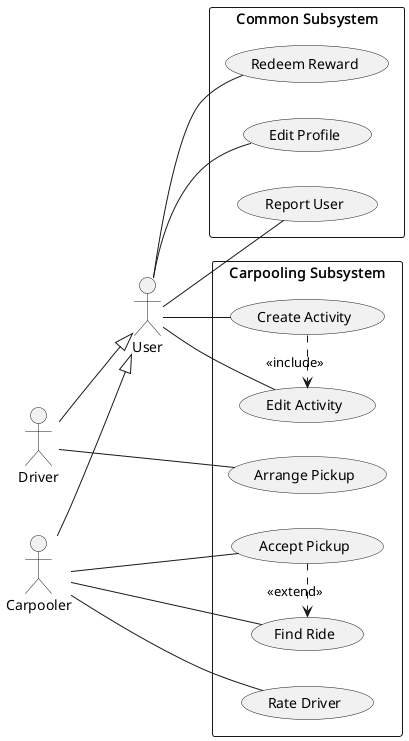
\includegraphics[width=\textwidth]{use-cases-carpooling}
    \caption{Use Case Diagram 1}
\end{figure}

\begin{figure}
    \centering
    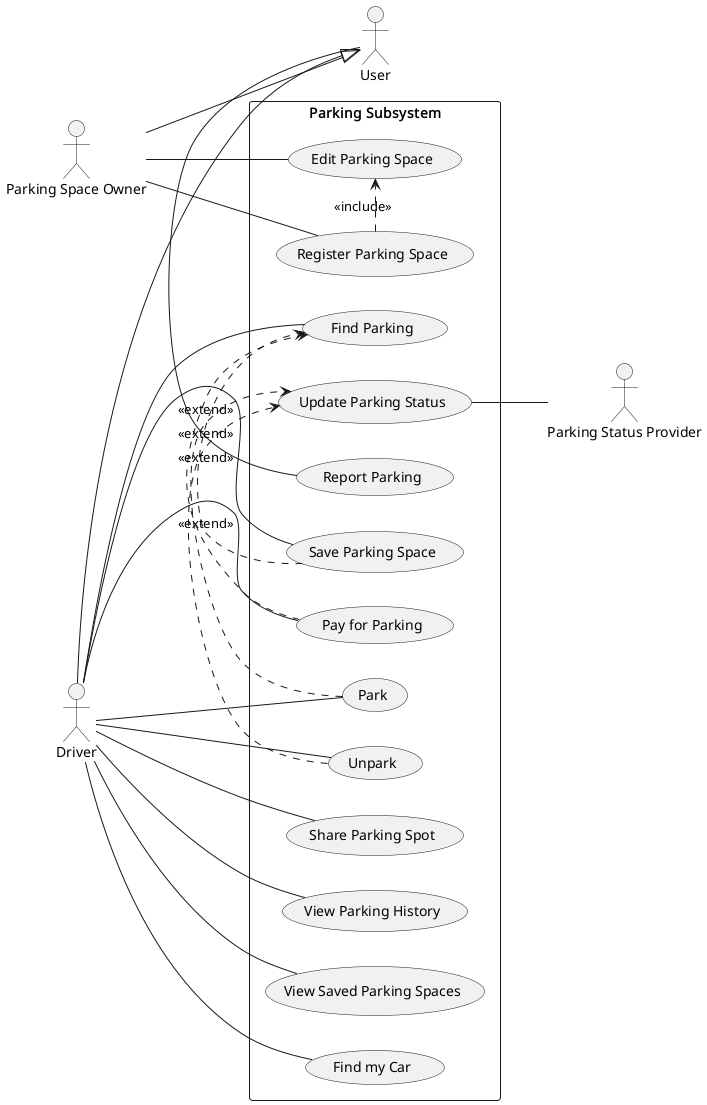
\includegraphics[width=\textwidth]{use-cases-parking}
    \caption{Use Case Diagram 2}
\end{figure}

\section{Απαιτήσεις και Προδιαγραφές}

\section{Χρήση Τεχνολογιών και Εργαλείων}

\end{document}
